\documentclass{cosart}
\begin{document}
\title{主站文章标题示例} % 填写文章标题
\arturl{http://cos.name/article-url/} % 填写文章的在线阅读地址 以"/"结束
\author{作者姓名} % 填写作者姓名
\authorinst{某某大学某某学院} % 填写作者单位
\maketitle
% title部分需要重新改写得更精致

\section{Section示例}

\subsection{Subsection示例}

\subsubsection{subsubsection示例}

惯例: section和subsection之间至少要有一小段文字, 效果不显突兀.

subsection和subsubsection同理. 行间公式示例: $e^{\pi i}=-1$.

图表交叉引用示例: (图\ref{fig1}, 表\ref{tab1}).

插图示例(PDF图形使用pdfcrop或Acrobat裁掉白边):
\begin{figure}[htbp]
\centering
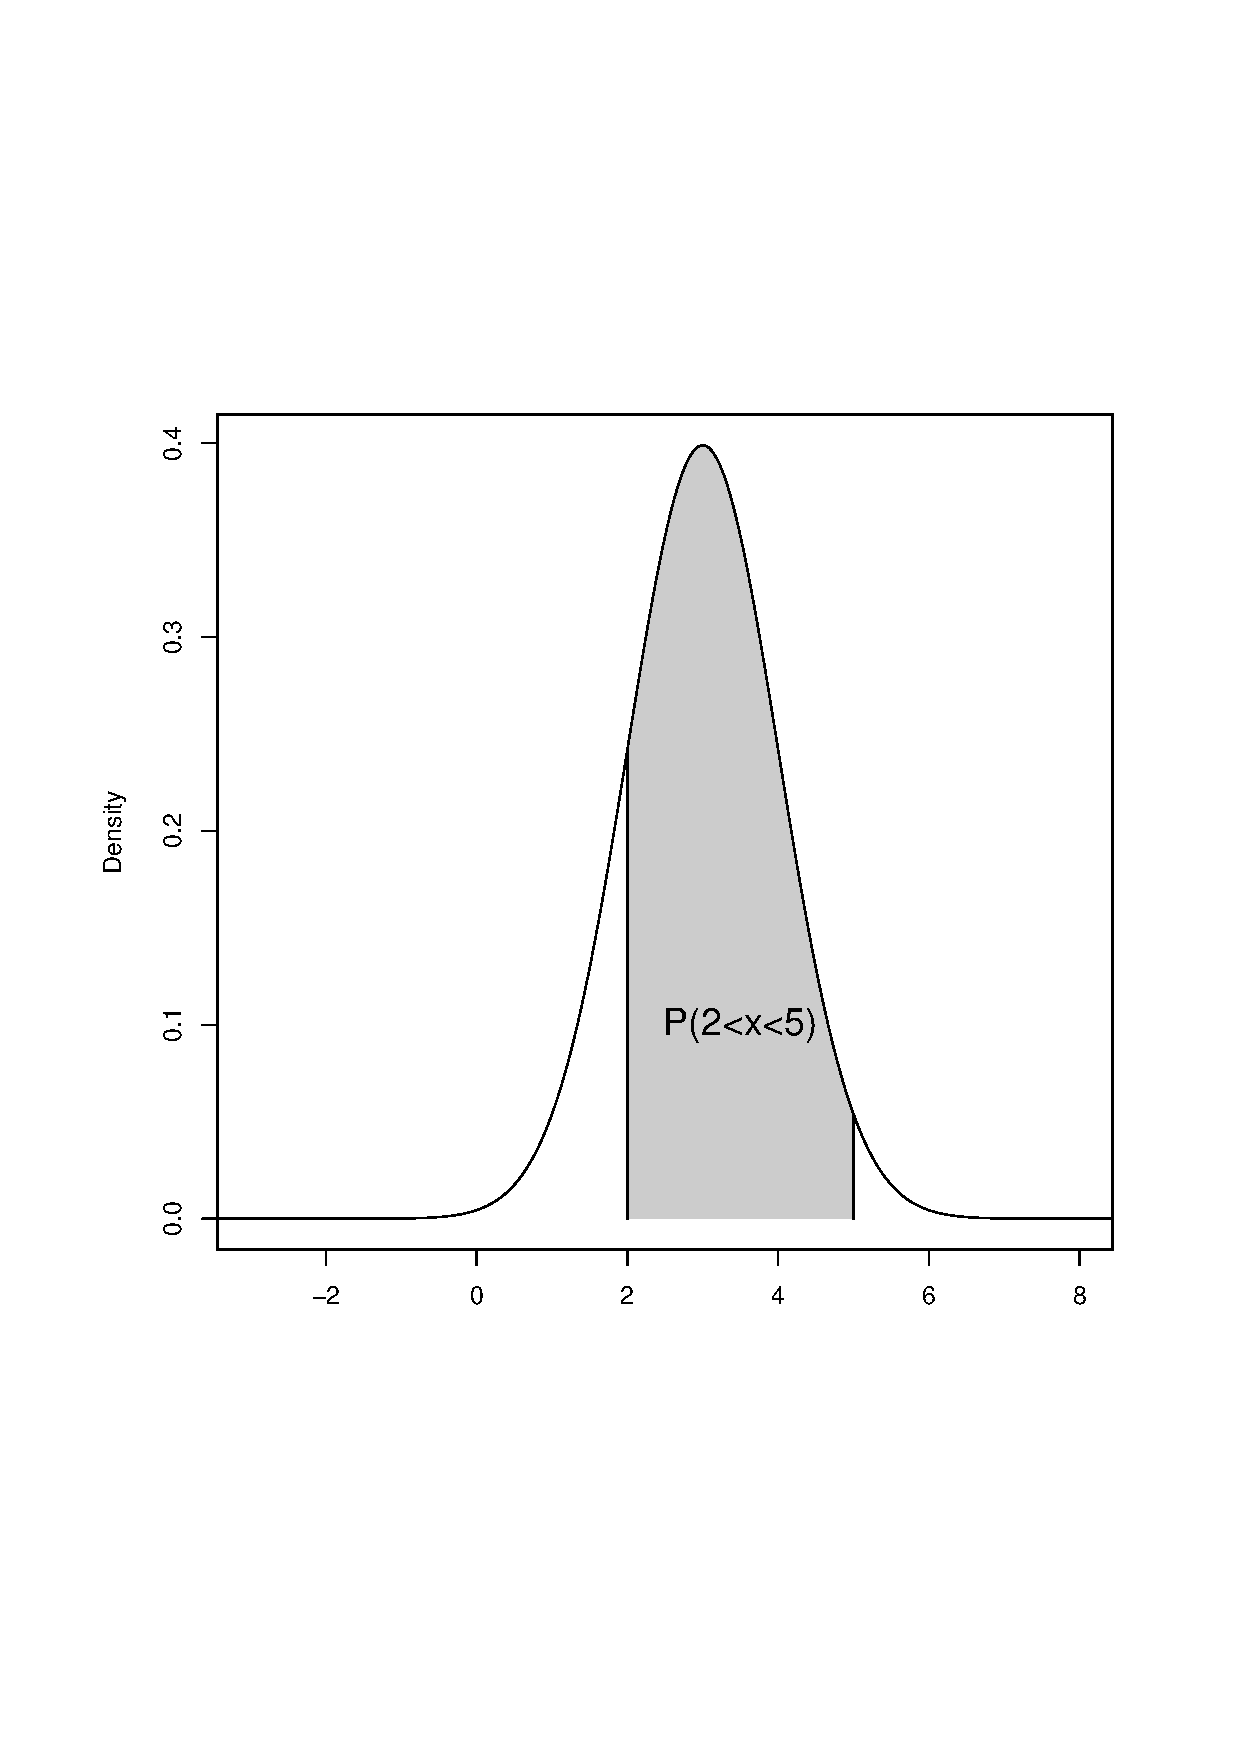
\includegraphics[width=0.65\textwidth]{figure.pdf}
\caption{$\lambda=10$, $\beta_1=0.1$, $\beta_2=0.2$的EWP分布} \label{fig1}
\end{figure}

三线表示例(自定义表格请使用相应宏包, 如tabularx和longtable):
\begin{table}[htbp]
  \centering
  \caption{三线表示例} \label{tab1}
    \begin{tabular}{cccc}
    \toprule
              & $-2\log(\Lambda)$ & 自由度$r$ & $p$值 \\
    \midrule
    标准泊松  & 2.69   & 1     & 0.1    \\
    EWP2      & 4.789  & 2     & 0.0912 \\
    EWP3      & 11.98  & 3     & 0.0075 \\
    CBR       & 10.764 & 4     & 0.0294 \\
    \bottomrule
    \end{tabular}
\end{table}

\begin{itemize}
  \item 项目1
  \item 项目2
  \item 项目3
\end{itemize}

\begin{enumerate}
  \item 带编号项目1
  \item 带编号项目2
  \item 带编号项目3
\end{enumerate}

\begin{description}
  \item[描述1] 详细描述1
  \item[描述2] 详细描述2
  \item[描述3] 详细描述3
\end{description}

有编号公式示例:
\begin{equation}\label{eqn_a}
  -\ln L(\lambda, \beta_1, \beta_2)=\beta_1\sum^{[\lambda]}_{k=x_{\min}}(\lambda-k) f_k+
\beta_2\sum^{x_{\max}}_{k=[\lambda]+1}(k-\lambda) f_k
\end{equation}

无编号公式示例:
\begin{equation*}\label{eqn_b}
  -\ln L(\lambda, \beta_1, \beta_2)=\beta_1\sum^{[\lambda]}_{k=x_{\min}}(\lambda-k) f_k+
\beta_2\sum^{x_{\max}}_{k=[\lambda]+1}(k-\lambda) f_k
\end{equation*}

需要对齐的长公式示例:
\[ \begin{split}
x=&a+b+c+\\
&d+e+f+g
\end{split} \]

无需对齐的长公式示例:
\begin{multline*}
x=a+b+c+\\
d+e+f+g
\end{multline*}

cases示例:
\[ \omega_k=\begin{cases}
e^{-\beta_1(\lambda-k)}, & k \leq \lambda\\
e^{-\beta_2(k-\lambda)}, & k > \lambda
\end{cases} \]

矩阵示例:
\[
\mathbf{Q}=\begin{pmatrix}
-\lambda_1 & \lambda_1 & 0 & \cdots & 0 \\
0 & -\lambda_2 & \lambda_2 & \cdots & 0 \\
0 & 0 & \lambda_3 & \cdots & \vdots \\
\vdots & \vdots & \vdots &  & \lambda_{n-1} \\
0 & 0 & 0 & \cdots & -\lambda_{n}
\end{pmatrix}
\]

行列式示例:
\[
\begin{vmatrix}
a_{11} & a_{12} & \cdots & a_{1n} & b_{1}\\
a_{21} & a_{22} & \cdots & a_{2n} & b_{2}\\
\vdots & \vdots &  & \vdots & \vdots\\
a_{n1} & a_{n2} & \cdots & a_{nn} & b_{n}
\end{vmatrix}
\]

需要对齐的公式组示例:
\begin{align*}
p'(t)&=\mathbf{Q}\,p(t)\\
p(t) &=c e^{\mathbf{Q}t}\\
p(1) &=c e^{\mathbf{Q}}\\
p(0) &=(1, 0, 0, \ldots, 0)
\end{align*}

不需对齐的公式组示例:
\begin{gather*}
a=b+c+d\\
x=y+z
\end{gather*}

并排插图 共享标题示例:
\begin{figure}[htbp]
\centering
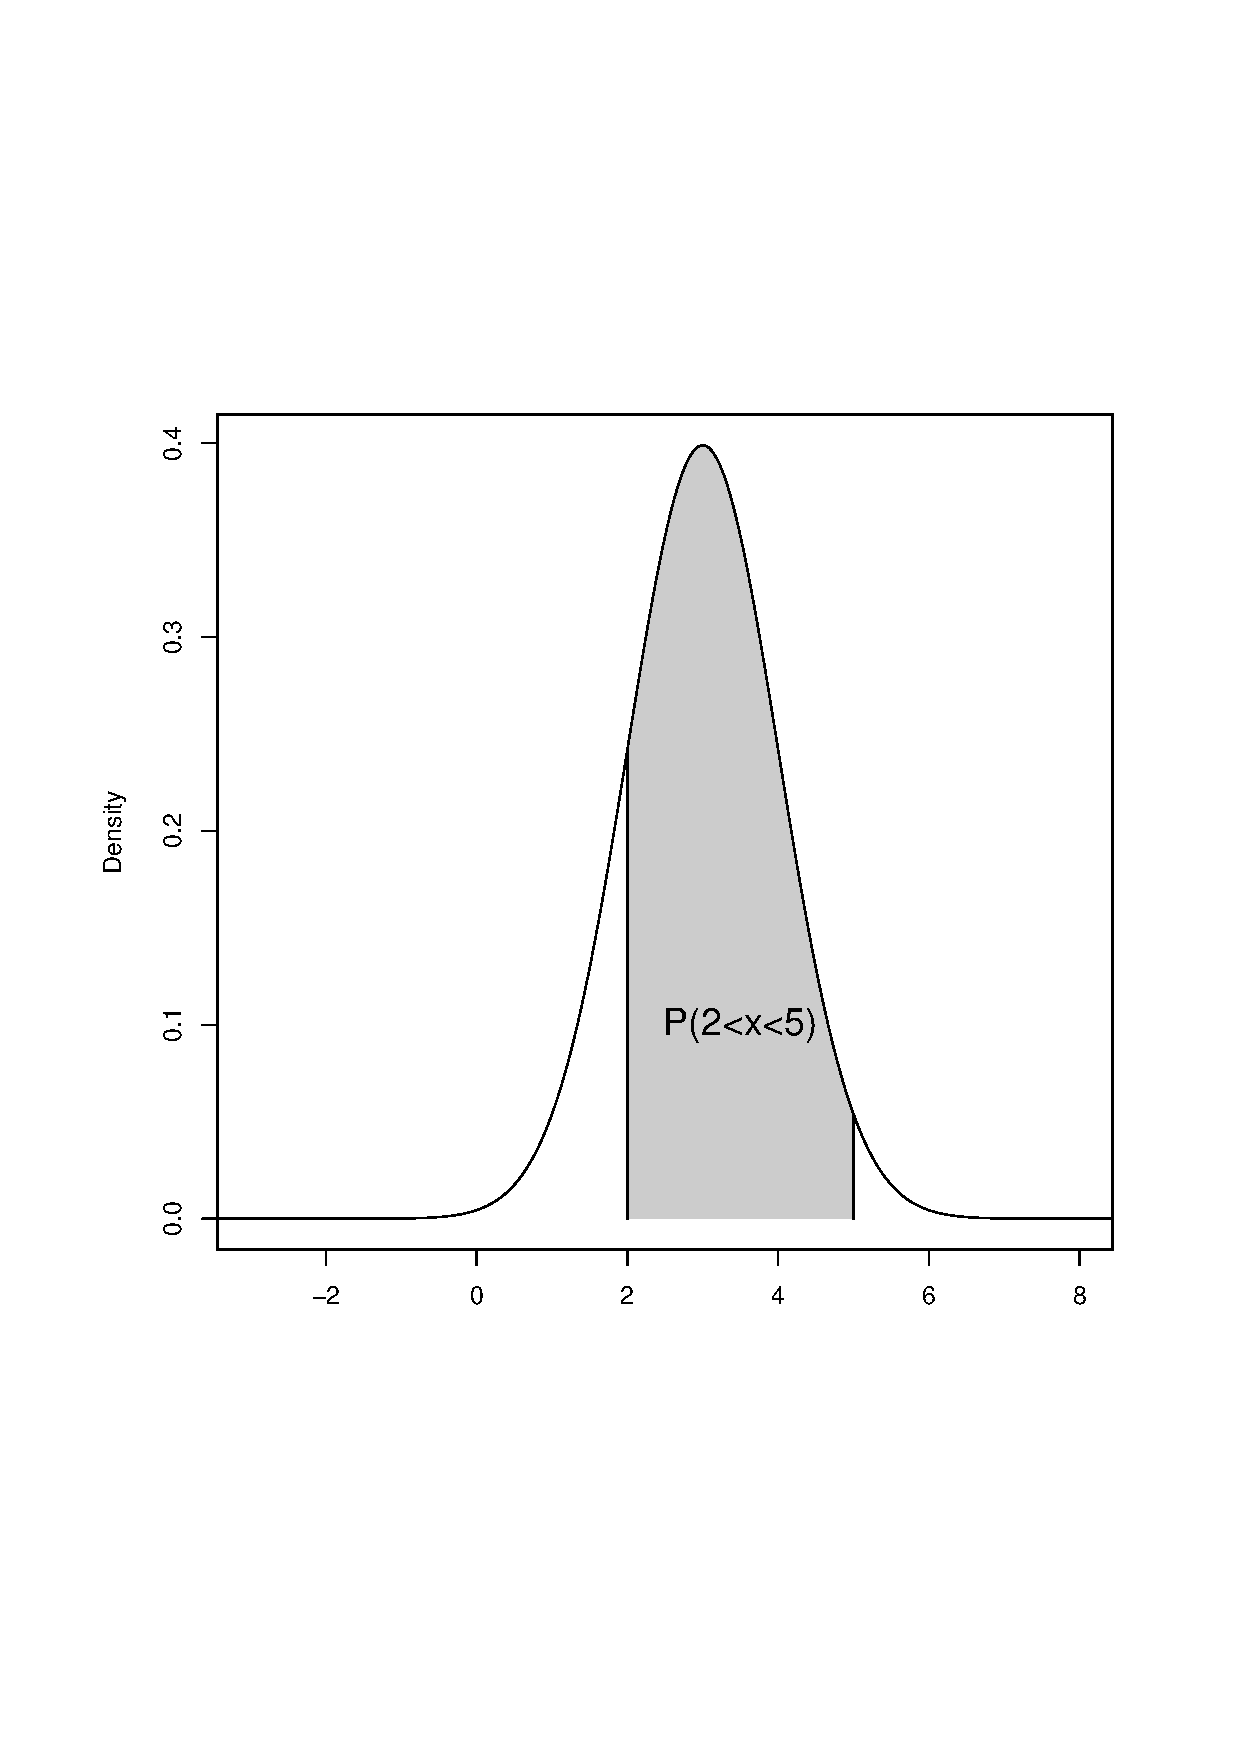
\includegraphics[width=0.40\textwidth]{figure.pdf}
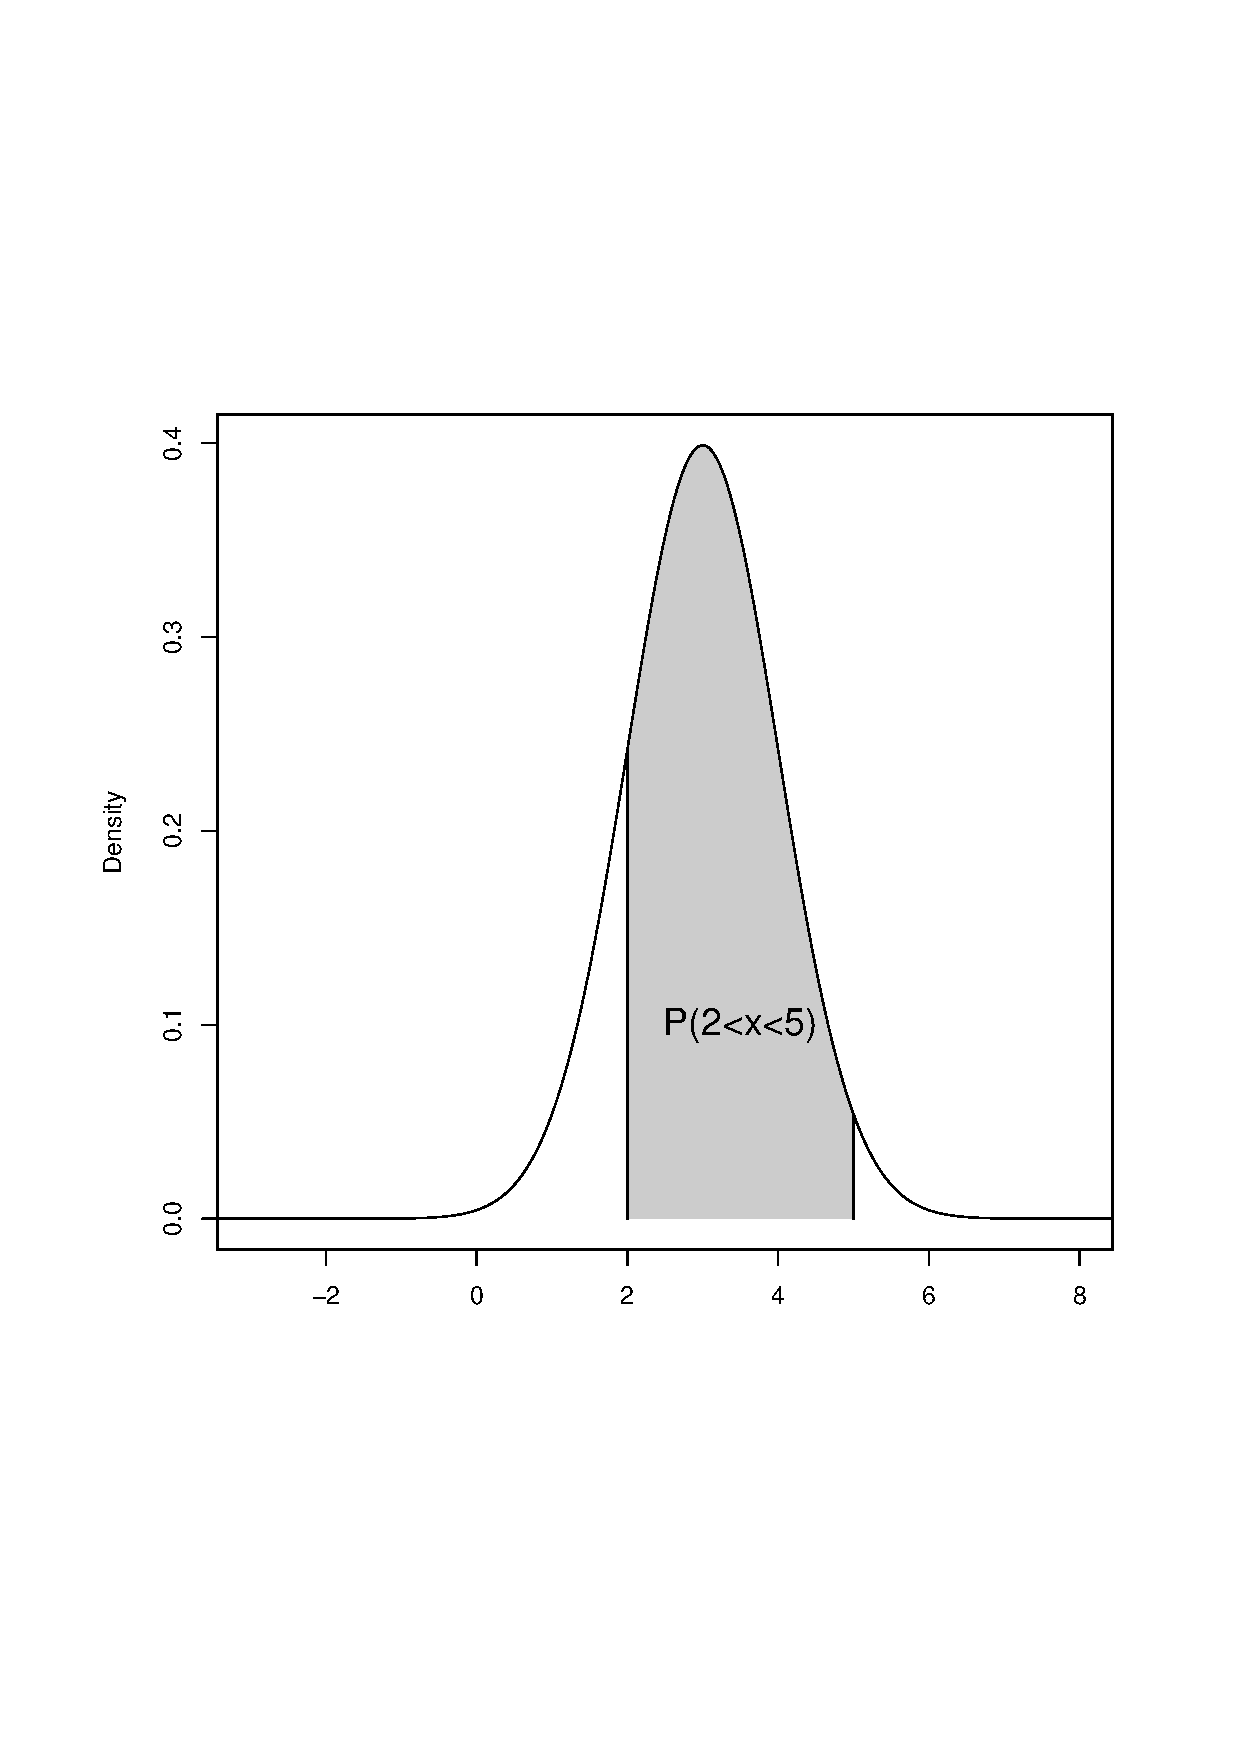
\includegraphics[width=0.40\textwidth]{figure.pdf}
\caption{并排插图, 共享标题}
\end{figure}

并排插图, 独立标题示例:
\begin{figure}[htp]
\begin{minipage}[t]{0.5\linewidth}
\centering
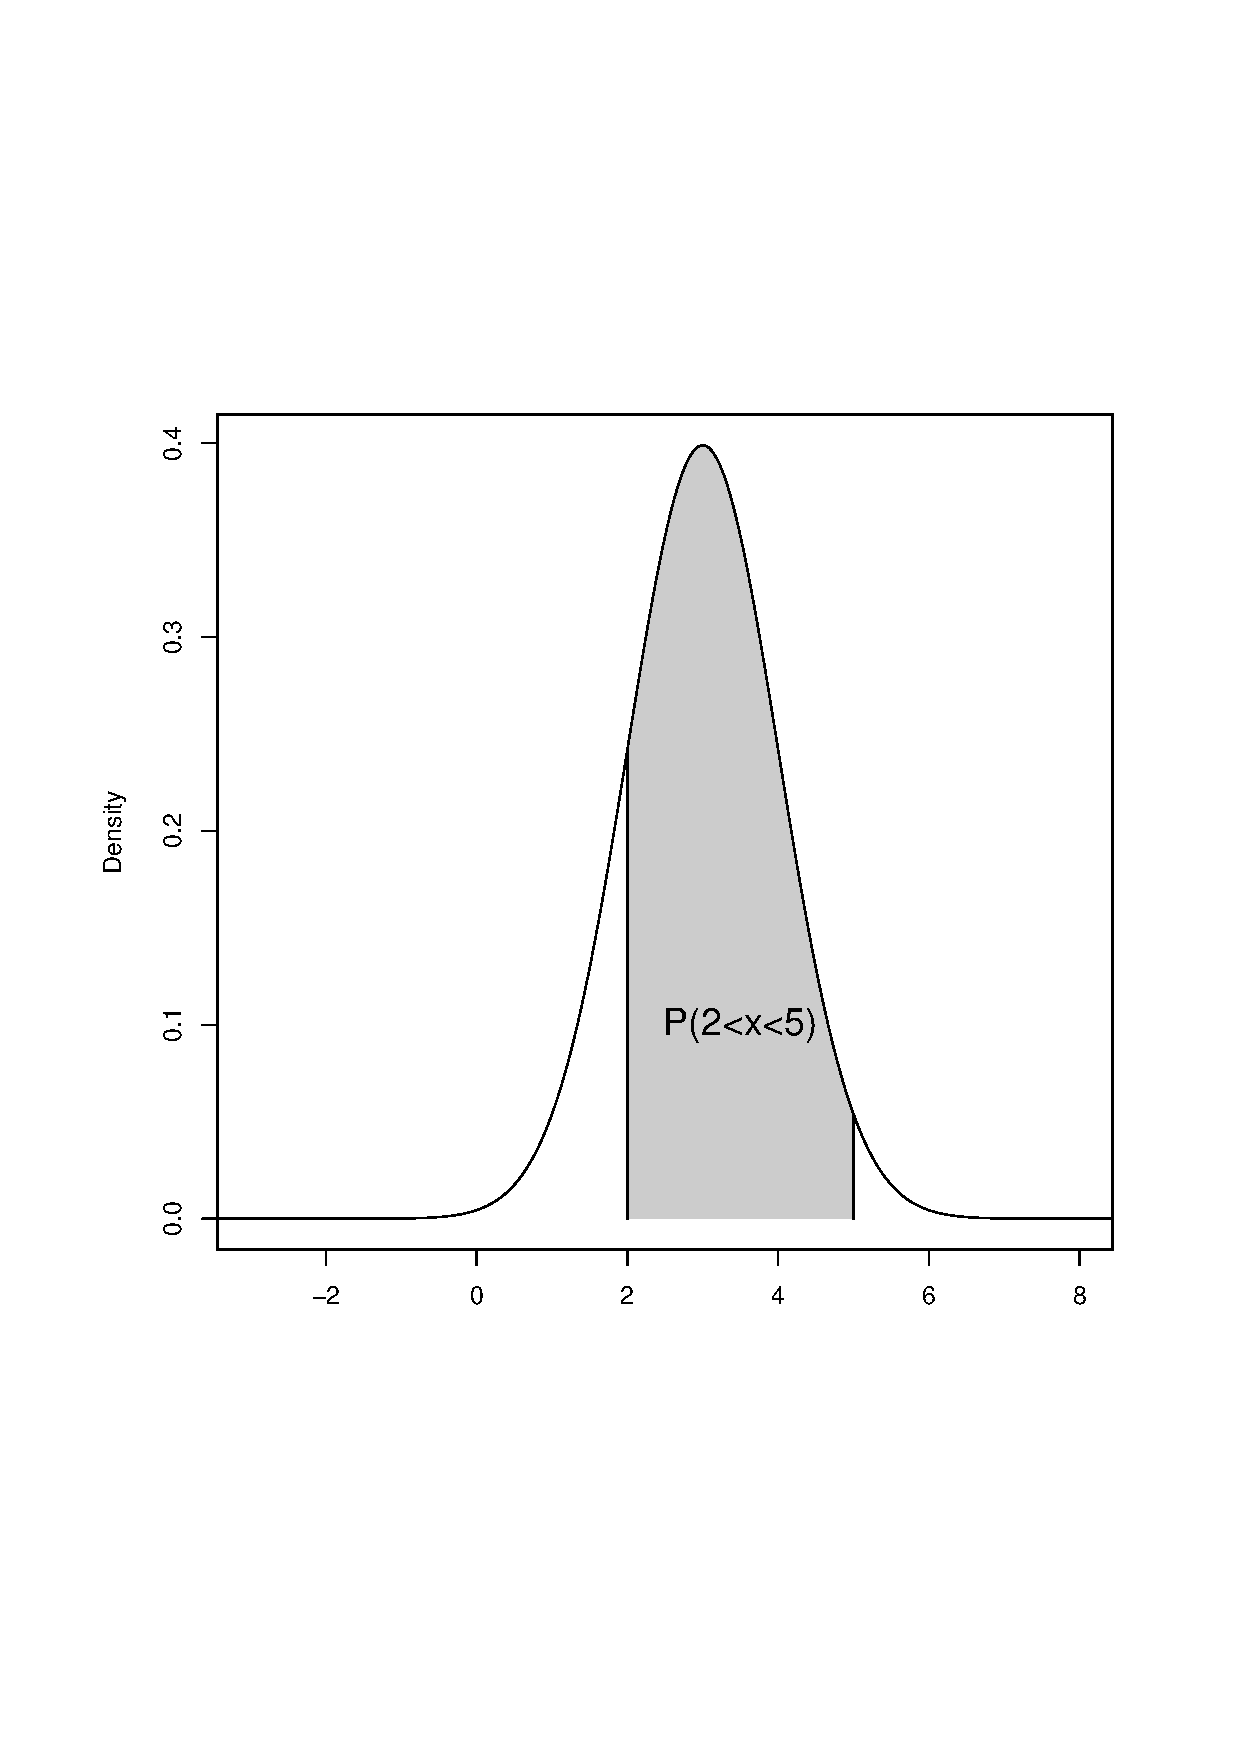
\includegraphics[width=0.80\textwidth]{figure.pdf}
\caption{左图} \label{fig:side:a}
\end{minipage}
\begin{minipage}[t]{0.5\linewidth}
\centering
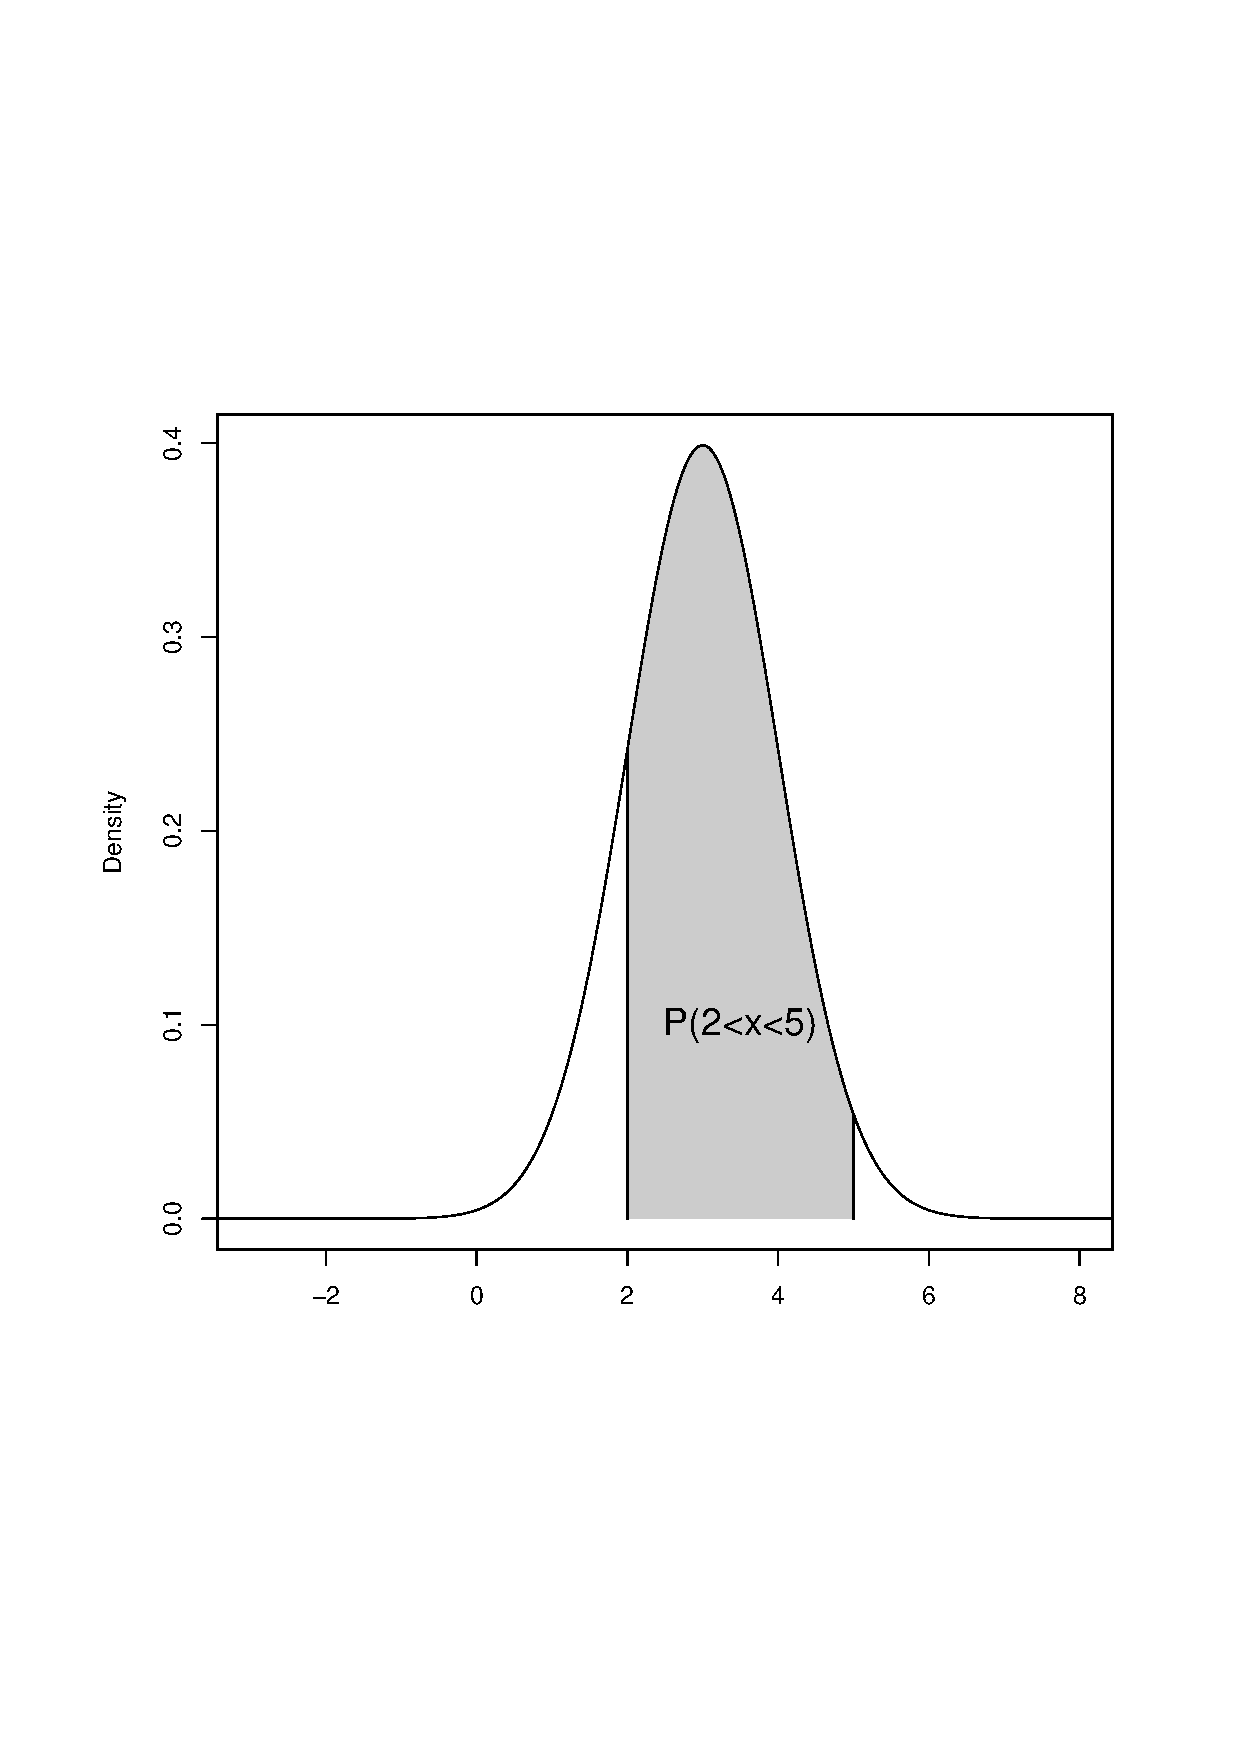
\includegraphics[width=0.80\textwidth]{figure.pdf}
\caption{右图} \label{fig:side:b}
\end{minipage}
\end{figure}

\begin{Verbatim}
# 代码环境示例 中英test混排
# Comments Here
library(foo)
foo <- function(x)
       {
       print(x)
       }
\end{Verbatim}

行间代码片段示例\rcode{test <- function(...){}}

编程语言名称示例:
\R , \prolang{C/C++}, \prolang{Python}, \prolang{Java}, \prolang{PHP}, \prolang{Haskell}.

包名称示例:
\pkg{stats}, \pkg{MASS}, \pkg{randomForest}

函数名称示例:
\fun{lm()}, \fun{kmeans()}, \fun{shell.exec()}

URL和E-mail地址示例: \url{http://cos.name/you-url/} \email{example@example.com}

俄文姓名示例: \font\fontWCA=wncyr10 {\fontWCA Kolmogorov}微分方程(Kolmogorov微分方程)

参考文献\citep{zhaokaihua1995}引用示例.

\nocite{*} % 显示未显式引用过的文献
\bibliography{cosart}
\end{document}
